%
% IEEE Transactions on Microwave Theory and Techniques example
% Tibault Reveyrand - http://www.microwave.fr
%
% http://www.microwave.fr/LaTeX.html
% ---------------------------------------



% ================================================
% Please HIGHLIGHT the new inputs such like this :
% Text :
%  \hl{comment}
% Aligned Eq. 
% \begin{shaded}
% \end{shaded}
% ================================================



\documentclass[journal]{IEEEtran}
\usepackage{emoji}
\usepackage[graphicx]{realboxes}
%\usepackage[retainorgcmds]{IEEEtrantools}
%\usepackage{bibentry}  
\usepackage{xcolor,soul,framed} %,caption
\usepackage{cite}
\usepackage{multirow}
\usepackage{fontawesome}
\colorlet{shadecolor}{yellow}
% \usepackage{color,soul}
\usepackage[pdftex]{graphicx}
\graphicspath{{../pdf/}{../jpeg/}}
\DeclareGraphicsExtensions{.pdf,.jpeg,.png}
\usepackage{caption}
\usepackage{subcaption}
\usepackage[cmex10]{amsmath}
%Mathabx do not work on ScribTex => Removed
%\usepackage{mathabx}
% \usepackage{algorithm}
% \usepackage{algpseudocode}
\usepackage{comment}
% \let\hl[1]\includecomment{#1}
\usepackage{enumerate}% http://ctan.org/pkg/enumerate

\usepackage[linesnumbered,ruled,vlined]{algorithm2e}



% % \usepackage
% \usepackage[ruled,vlined]{algorithm2e}
% \DeclareMathOperator{\ind}{ind}
% \DeclareMathOperator{\val}{val}
% \DeclareMathOperator{\ptr}{ptr}
% \DeclareMathOperator{\row}{row}
% \usepackage{algpseudocode}
\hyphenation{op-tical net-works semi-conduc-tor}

%\bstctlcite{IEEE:BSTcontrol}


%=== TITLE & AUTHORS ====================================================================
\begin{document}
\bstctlcite{IEEEexample:BSTcontrol}
    % \title{Adversarial attacks on federarted learning for medical image analysis}
    \title{Adversarial attacks on federated learning networks for medical image analysis}
  \author{Erfan~Darzi,~\IEEEmembership{Student Member,~IEEE,}
      P.M.A van Ooijen,~\IEEEmembership{Senior Member,~IEEE,}
    %   and~Zoya~Popovi\'c,~\IEEEmembership{Fellow,~IEEE}% <-this % stops a space

  \thanks{ This paper is being prepared with IEEE standards This work was funded in part by NWO under project AMICUS}
  \thanks{Erfan Darzidehkalani is with UMCG (e-mail: e.darzidehkalani@umcg.nl).}% <-this % stops a space
  }

% The paper headers
% \markboth{IEEE TRANSACTIONS ON MICROWAVE THEORY AND TECHNIQUES, VOL.~60, NO.~12, DECEMBER~2012
% }{Roberg \MakeLowercase{\textit{et al.}}: Cross modality image transformation using cyclic residual
% architecture and evolutionary algorithm}


% ====================================================================
\maketitle



% === ABSTRACT ====================================================================
% =================================================================================
\begin{abstract}
%\boldmath
Federated learning (FL) can significantly mitigate privacy concerns for Medical image analysis (MIA) systems. However, its decentralized and collaborative nature can bring new attack surfaces which might impose severe threats for participating clients.  
This paper investigates adversarial attacks where the adversary tries to fool other clients with manipulated data. 
% We presume a differentially private setting where the adversary has no access to other clients' models and data.
We investigate the credibility of known threat factors in a federated environment and discuss their importance. We demonstrate that domain-specific settings can lead to higher attacker success on MRI tumor and pathology imaging datasets.
In addition, we propose a scenario in which the adversary leverages the federated environment to devise a more powerful attack. We show that using gradient information from previous global model updates enables single-step attacks (e.g., FGSM) to outperform computationally expensive iterative methods so that the adversary reaches the same success rate $20 to 30$ times faster.
\end{abstract}



% === KEYWORDS
% ====================================================================
% =================================================================================
\begin{IEEEkeywords}
Adversarial attacks, Federated learning, Medical imaging, Deep learning
\end{IEEEkeywords}






% For peer review papers, you can put extra information on the cover
% page as needed:
% \ifCLASSOPTIONpeerreview
% \begin{center} \bfseries EDICS Category: 3-BBND \end{center}
% \fi
%
% For peerreview papers, this IEEEtran command inserts a page break and
% creates the second title. It will be ignored for other modes.
\IEEEpeerreviewmaketitle


% ====================================================================
% ====================================================================
% ====================================================================










% \tableofcontents
% === I. INTRODUCTION =============================================================
% =================================================================================
\section{Introduction}
\IEEEPARstart{I}n the past few years, federated learning (FL) has emerged as one of the mainstream machine learning (ML) paradigms and gained much attention in the field of medical image analysis (MIA). Federated learning enables hospitals and other healthcare providers to train machine learning models jointly with other hospitals without sharing sensitive data. It is applied to a wide scope of MIA tasks, successfully addressing data governance concerns. Notable works include brain tumor classification and segmentation, breast density classification, and covid-19 detection. \cite{sheller2020federated,dayan2021federated,rieke2020future}.



Although FL has mitigated many risks and concerns about multi-institutional collaborations, it is still vulnerable to other privacy issues. Several emerging attacks are proven to threaten FL networks. Adversarial clients might be able to change the model's prediction or gain information about other clients by actively changing its own model parameters or synthesizing fake input data.





This paper analyzes a group of attack scenarios called 'adversarial attacks.' A malicious client aims to cheat the model by adding subtle noise to its examples. The noise is so minimal that the change in the image is imperceptible for a human observer. However, it can cause the model to misclassify it. 
Adversarial attacks are the main source of vulnerability to the deployed FL models \cite{bouacida2021vulnerabilities,lyu2020threats,costa2021covert,lyu2020privacy}\. and are designed to fool the models that  are already trained 
% So their threat for the deployment phase 
passed their test phase and delivered for clinical use. 
% \\Although there is some research in the past in FL and MI, we believe that adversarial attacks could also be explored since they could be a threat to clinical decision-making.
% \\The attacks are analyzed in a federated setting to investigate their inter-client transferability.
\\We leverage the FL environment to propose a stronger attack and show that it enables adversarial clients to manipulate other benign clients to a high degree.  
We also show that proposed defense methods such as differential privacy still have limited effect against this attack.
In the following sections, we introduce adversarial attacks, sources of vulnerability, and our method.

\begin{figure}[t!]
 \centering
 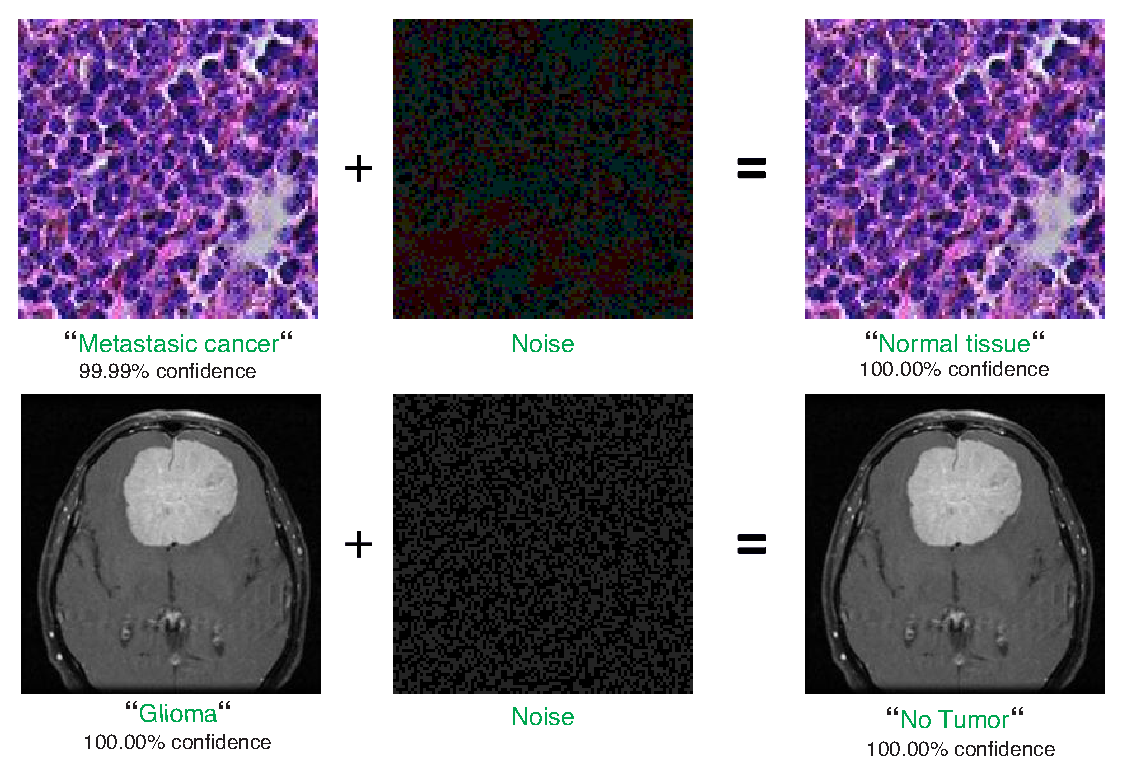
\includegraphics[width=0.52\textwidth]{Whatisads.eps}
 \caption{A schema of adversarial attacks to cancer detection systems}
 \label{fig:pgd-atta-comparison}
\end{figure}
 
 
% We argue that federated MIA systems, besides being susceptible to the known security and privacy vulnerabilities encountered in typical ML settings  FL and MI each expose new attack surfaces.

% Pretrained models are mostly used by radiologists and are integrated in the medical imaging software.
% These crafted images can change the model output to deceive the end-users of deep learning models (i.e. clinicians), so they could be directly affect clinical decision making. 
% The adversary can similar attacks during the training phase, but these attacks vurnelable  and is deployed. This is especially important since in training phase attacks, the adversarial client is under continious communication with the central server. And there are 



% clients trying to fool images during the training stage where  where the trained model is deployed in hospitals for clinical usage.

% It is a passive attack meaning that the adversarial client can train the model in a normal way so that current defense ways are unable to detect if a client is trying to do an adversarial attack.


%  Even if in indirect use and as a backbone for imaging software.
 \subsection{ Adversarial attacks }
Adversarial attacks are attributed to the linear characteristics of high-dimensional data. \cite{goodfellow2014explaining}. The crafted noise examples produced using one model might be able to manipulate other models. In FL setting, these attacks are also known as evasion attacks.\cite{biggio2013evasion,costa2021covert,ayub2020model,bouacida2021vulnerabilities}, are defined as if a malicious client tries to manipulate other clients with fake data.\\
At the same time, research on defense methods is also ongoing. Some studies tried to incorporate differential privacy (DP) as a protection measure in FL setting. Differential privacy was initially proposed to protect against privacy attacks, but it has also been applied against adversarial attacks.\cite{bouacida2021vulnerabilities,asgari2018vulnerability,wu2020evaluation}. Despite the ongoing research, there is no universal defense method against them.

We have introduced adversarial attacks in the scope of FL and MIA systems. We argue that distinct features of FL environments and MI make their combination highly vulnerable to adversarial attacks. \cite{chen2017targeted,chen2019deepinspect,ji2018model}.  The following paragraphs argue how each FL and MI expose new attack surfaces.
\\\textbf{Federated learning and adversarial attacks:} FL characteristics are known to elevate the impact of attacks known in the centralized setting. \cite{goldblum2020dataset,liu2022threats} The unique vulnerabilities of FL can be :
% We think the adversarial attacks on federated learning medical systems are notable important for three reasons, and this topic might not be explored properly. 
\begin{enumerate}[(i)]

\item{\textit{More data:} }
Each model received in every round has updated information about other clients. Adversaries can exploit this information to prepare stronger attacks.\cite{sun2019can,fang2020local,wang2020attack,song2020analyzing}
\item \textit{Open training:} In FL, the training process involves a lot of participants. Among them, one adversary could act maliciously.
\item{\textit{Standardized data pipelines:}} FAIR data stations and data standardization steps are inherent in many of FL networks in hospitals\cite{wilkinson2016fair}, near Global 
Electronic data management and medical communications (DICOM) integrated into the federated pipelines.
\cite{van2022ai}. Clients with more similar data are prone to attacks. \cite{miotto2016deep}
\item \textit{Scale of deployments:} FL networks have been deployed on a large scale in healthcare. Models act as a backbone of multiple inference software. FL networks in the deployment stage are especially weak against adversarial attacks. \cite{costa2021covert,bouacida2021vulnerabilities}.

\end{enumerate}
\textbf{Medical images and adversarial attacks}: Also, medical images have distinct features which makes the networks trained on them more vulnerable.
\begin{enumerate}[(i)]
    \item {\textit{Feature representation:}} Due to the inherent feature space of medical images, MIA systems are more vulnerable to this sort of attack than natural images. As shown in  previously published work, medical images have a narrower high-dimensional feature representation of images than natural images, causing trained networks to be over-parameterized. \cite{ma2021understanding} Over-parameterized networks are inherently easier to fool. \cite{Ye_2019_ICCV} As a result, medical imaging classifiers are easier to fool than natural image classifiers.  \cite{ma2021understanding} Several works have confirmed this by arbitrarily manipulating Funduscupy, Chest X-Ray and Dermoscopy data resulting in ... \cite{finlayson2019adversarial}. 
    \item \textit{Unique texture:}Medical images have limited texture diversity, and small texture perturbation in medical images can confuse classifiers to a high degree. \cite{ma2021understanding} This feature can be of advantage to the adversary's attacks, because they can perturb the texture in irrelevant areas and fool the classifier without manipulating the more important parts, e.g., the tumor area.\cite{ma2021understanding}. Which has, for example, been shown to effectively confuse tumor detection classifiers  \cite{gupta2022vulnerability}
    
\end{enumerate}



\subsection{Transferability factors}
Despite defense not always being an option, DL systems might be able to gain insight into their points of vulnerability. Some parameters and deployment settings might increase the chances of a successful attack.\\
Gaining such perception can be directly imported in security analysis so that the technicians know where the highest threat can be from, and they do not require a brute-force simulation of all the scenarios and parameter values, which is practically hard and in most cases impossible. 
\\The research is ongoing on attack transferability.\cite{gao2022boosting,elaalami2022bod,dai2021fast,duan2022novel,du2020hybrid,zheng2020efficient,shafahi2019adversarial,qiu2022framework}. In the MIA domain, transferability analysis has been done in a centralized ML setting, and the results are found to be domain specific. Factors such as data disparity, perturbation degree, and pre-training are shown to be crucial in attack transferability. However, their extent and optimal values might vary to a large extent. This difference can be attributed to the characteristics of the target imaging domain, texture of images, and whether the attack is white-box or black-box.\cite{ma2021understanding} \cite{bortsova2021adversarial}. \\ In an FL setup with a higher level of complexity, their findings might have limited pertinence. \cite{costa2021covert} One research question could be how FL can bring up new factors, and whether its optimal attack settings are concordant with the existing literature obtained from centralized data experiments. 
In this project we investigated potential factors in this setup, and discuss their effect on transferability.




\\\subsection{Our attack}
%  One question might be whether if an advesary can leverage  a federated setting
%  faster attacks? What could  Escpeciially in
% ÷/here the adversarial client might incorporate its additional knowledge to prepare better attacks.
%  We use the  
% More importantly, 
% An adversarial client is not in direct contact with the surrogate models,
% however, In the traditional FL where each client receives a similar final global model an adversarial example trained on one client can be applied to any other client.
% It is shown that of FL networks are vulnerable to adversarial attacks is when deployed as a service to end-users.  \cite{costa2021covert,bouacida2021vulnerabilities}. And adversarial attacks are the main source of vulnerability to the deployed FL models.\s
% Attackers might be able 

% \textbf{Transferability / stacking}
% White box attacks on Federated learning networks, the adversary has complete knowledge about other clients network architecture, gradients and parameters. In blackbox setting, however, the adversary does not know about other clients weights. 
% a ifferentially private settings,
% where individual clients are separated so that each client's privacy is guaranteed, and
% where communication are noisy-double sided to make any attack black-box,
% \textbf{Cross-round noise}
% Simply using gradient values might result in drastic change, so the this method might not be always feasible\cite{zhang2019theoretically} \cite{pan2019improving} \cite{zheng2020efficient}.  
% periodically resetting the input gradients has been studied  \cite{zheng2020efficient} has been investigated in adversarial training, however, it results in loosing gradient information. 
The adversarial client participating in an FL setup has access to previous model updates. We investigate a scenario where the adversary can enhance its attack using the gradient information from those model updates. However, obtaining gradient information might be a challenge, and also transferring them to the subsequent models causes drastic parameter change.\cite{zheng2020efficient}
We introduce an intermediary noise tensor we call \textit{Cross-round noise (CRN)} which utilizes previously received global model updates to generate noise and passes them to the next FL round. To initialize the next round and avoid parameter change, we regularize $L_{2}$ each noise channel by its mean value. 
\\This way can achieve better performance and improve transferability, with a much lower computation burden than the standard attack methods. %This can boost the computationally expensive attack models and bring higher capability.

% We assumed that the attacker doesn't necessarily have knowledge about model weights or inner settings of the target model, or the softwares that are build upon the model.\\




% \hl{

% Adversarial attacks are important in MEDICAL IMAGING  FL and not other attacks
% }

% \hl{tozieh bede ke chera evasion attack ro entekhab kardi va rabtesh be medical chie (masala model poisinning ya free rider chera na)}


% There are other manipulations but we chose adversarial attacks.
% 1- they preserver content
% 2- they designed for fool end-users and deployment.

% Like there are several attacks that can 
% causes the model not to converge or fail. 
% Other types of manipulations exist in the literature. Adversarial attaks are important for some reaasons, first, they aim presesrve the content of the image and the attack is imperceptible by human.% FL are more vulnerable during test phase.Mostly because a test phase before development can reveal impaired mod
%  In the medical imaging context, the deployment phase attacks are designed to manipulate the end-users, rather than hampering the training process. Adversarial attacks are only designed for the deployment phase, and are the only verified source of vulnerability of deployed FL models.el.
% Although but adverIt can impact clinical decision making. 
% the attacks during deployment phase % various reasons. Failure of models, communication bottlenecks, dropout of clients, non-robust aggregation, and poisoned model updates. 

% % Federated networks can be attacked during development or deployment phase. Here we focus on 
% Adversarial attack aim the end-users, \cite{ Vulnerabilities in FL}  after the model has passed its test phase. In the clinical setting, these manipulation to a federated network that could have directly impact the clinical desicion making.  Other forms of manipulations to FL exist. As an example failure of models, communication bottlenecks, dropout of clients, non-robust aggregation, and poisoned model updates can hamper the training proces



\\
\subsection{Organization of paper}


This paper evaluates the effect and degree of adversarial attacks on DP-enabled FL networks in MIA. To our knowledge, this is the first time malicious attacks are analyzed in federated MIA networks. We performed the most common attacks, namely PGD, basic iterative, and FGSM methods. Adversarial attacks are an essential threat to deep learning networks and significantly decrease performance. This is especially important in the MIA, where FL-trained networks are deployed as a tool to diagnose and analyze. We also assumed that some parameters might be essential to determine how transferable the attacks are, namely, the degree of perturbation and iteration steps. Which is not fully explored yet. We think that these parameters are vital since they balance the compromise between the imperceptibility of the noise and the success of the attack.\\ The study is done to detect cancerous images, namely GLioma, Meningioma, and histopathology. Tumor type classification is a multi-class classification of tumors in a setting with three participating hospitals. We did it with SOTA deep learning modes and discussed the importance of each potential factor in a DP-enabled environment. And discuss the provided model of attack.
%To the best of our knowledge, no study has investigated the scenarios for MIA.



We can summarize our contributions as follows.

\begin{itemize}
  \item To the best of our knowledge, this is the first study introducing and investigating adversarial attacks on FL in the MIA. We discuss its importance for the medical imaging society, potential real-world threats, and implemented attack scenarios.

\item We test and compare the popular attacking methods on a DP-enabled setting, where DP requirements are imposed on both sides of the communication. Although some studies have adversarial attacks in medical imaging, None has investigated them in a differentially private setting.

  \item  We introduce a new attack and show the superiority of our model compared to the popular models. We show that sometimes single-step calculation can outperform computationally expensive models.
%   \item We discuss how unexpolored parameters can play in this setting and affect the transferability, and perceptibility.
    \item We discuss how domain-specific parameters can affect the transferability ,and try to estimate their optimal values in our setting. We calculate attack success rate and error transfer rate in each medical imaging task.
  \item We do all of the above on popular MIA datasets and tasks, namely detecting and classifying cancer in brain MRI and histopathology images
  
\end{itemize}


The rest of paper is organized as follows, the next section discusses adversarial attacks on MIA and FL systems. Section \ref{sec:prelimianries} introduces FL, differential privacy and attack models,  \ref{sec:attack} introduces our attack method. Next section introduces our attack, results and then discussion and the last section will be conclusion.
% \\\hl{bishtar dalil mituni biari ke chera taeene levele noise mohemme wa chera in parametera ehtemalan moheman va bayad baresi beshan }
% \hl{\\ We study effect , number of participants, chera mohemme (ba literature sabet kon)}\\
% \hl{\faClockO  Adv attack Is not noise}\\
\section{Background and Related works}

 % $\Delta W_n^t$
 
Federated learning has demonstrated efficacy in an array of imaging modalities, including Magnetic Resonance Imaging (MRI) \cite{sheller2020federated}\cite{silva2019federated}, X-ray \cite{balachandar2020accounting}, retinal imaging \cite{balachandar2020accounting}, as well as in applications such as brain tumor segmentation \cite{bakas2017advancing}\cite{lee2018privacy}, diagnosis \cite{pan2019improving}, and treatment selection \cite{lee2018privacy}. In particular, Federated Learning (FL) has proven to be a valuable tool for supporting physicians in their decision-making process regarding the treatment of COVID-19 patients. A landmark study that involved 20 institutions across five continents found that FL played a significant role in shaping patient treatment plans\cite{flores2021federated}. The study employed chest radiography images in conjunction with clinical information to determine the appropriate level of care and oxygen requirements for patients afflicted with COVID-19. It was observed that FL improved the performance of the predictive model, especially for institutions with smaller datasets, compared to using only local data for model training. Additionally, it was found that healthcare facilities with smaller datasets often had underrepresented categories due to a low number of patients in certain classes. The implementation of FL led to a notable improvement in predictions for these underrepresented patient categories.

\begin{figure*}[t!]
\centering
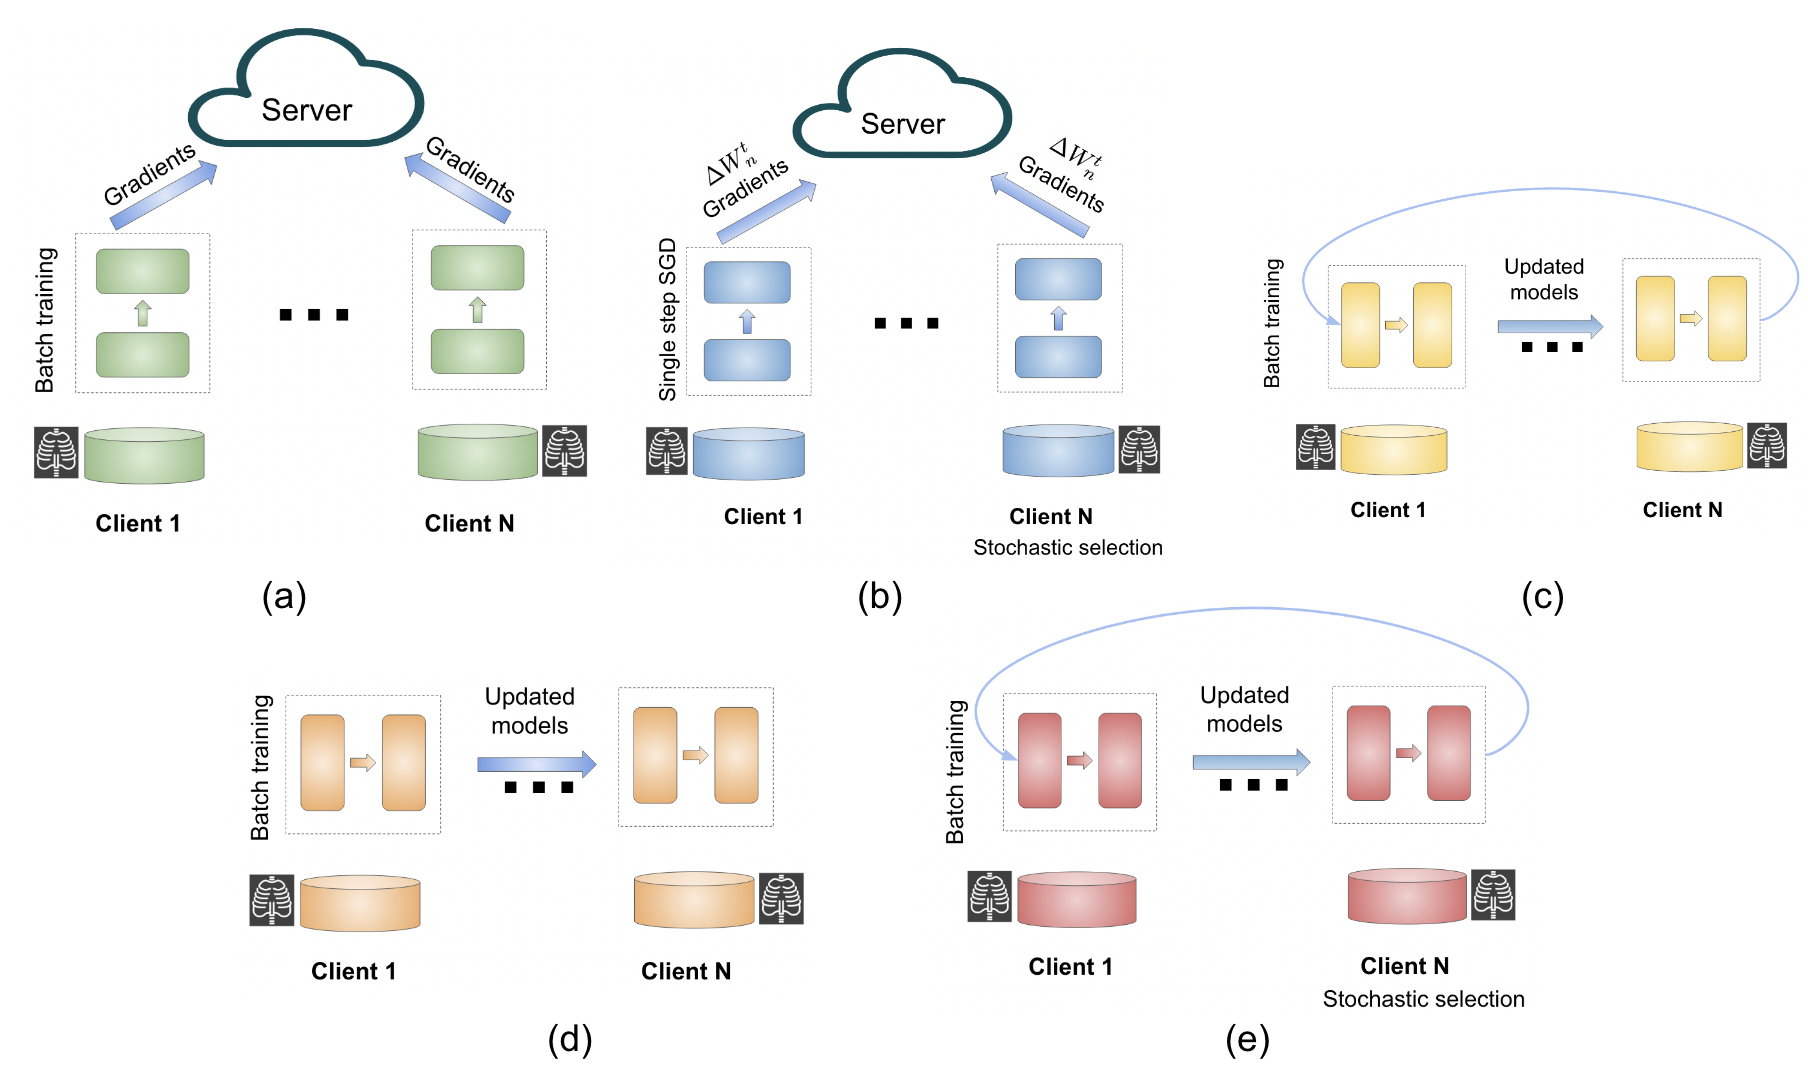
\includegraphics[width=1\textwidth]{FLmodels.png}
\caption{Illustration of FL models and algorithms: (a) Federated averaging, where clients train on a local batch of data. (b) FedSGD, in which a subset of clients is selected, and each performs a single step of SGD before sending model updates to the server. (c) Cyclic Weight Transfer (CWT), where clients train locally and pass the model to the next client, repeating the cycle. (d) Single Weight Transfer (SWT), where the model passes through each client only once. (e) Stochastic Weight Transfer (STWT), in which the model is sequentially passed through clients, with participating clients in each round being sampled randomly.}
\label{fig:flalgorithms}
\end{figure*}


Recent research has focused on the classification of scan images to distinguish between COVID-19 patients and healthy individuals, as well as identifying lesion areas. The primary application of AI in managing COVID-19 patients has been the interpretation of radiology images, especially chest CT scans.  The detection of lung alterations through these scans plays an important role in optimizing patient management and guiding treatment decisions\cite{yan2020interpretable}\cite{hu2020challenges}\cite{burian2020intensive}.  Several studies have also explored 3D Convolutional neural networks \cite{wang2020weakly} and COVID-19 detection with a limited number of training samples.

While the majority of these studies report favorable accuracy, they often presume a centralized environment wherein a single data center has access to all data. However, a few studies have successfully applied distributed learning for COVID-19 detection, employing global aggregation models such as model averaging in federated learning settings\cite{ho2022fedsgdcovid}\cite{zhang2021dynamic}, or within a blockchain framework \cite{kumar2021blockchain}. These studies have pointed to certain limitations of existing algorithms, such as high communication overhead \cite{remedios2020federated}, as well as convergence issues or catastrophic forgetting when the number of participating hospitals increases \cite{sheller2020federated} \cite{chang2018distributed}.


To our knowledge, no study has been performed that compared multiple FL algorithms under standard conditions to evaluate their applicability. Therefore, comparing multiple FL algorithms under standard conditions could be informative in evaluating their applicability in practice.

To evaluate the existing methods from multiple perspectives, we have implemented the most popular models and compared them in terms of performance, communication overhead, and computation burden.
\section{Preliminaries}
\label{sec:prelimianries}
\subsection{Federated Learning}



Federated learning enables multiple data owners with private datasets to jointly train a global model based on local models. The  optimization problem could be formulated as
${w} = \sum\limits_{i=1}^{N}{p_{i}{w}_{i}}$ , ${w}_{i}=\arg\min\limits_{{w}_{i}}{\left(\mathcal{L}(\mathcal{D}_{i};{w})\right)}$ where $N$ is the number of data owners, $\mathcal{L}(\mathcal{D}_{i};{w})$ is a loss function indicating global model parameters  ${w}$ of local datasets.  
 The learning procedure is an iterative process containing local and global steps. Each data owner trains a global model on its local dataset received from a global server in local iterations. The global server aggregates the updated local models for the next round for updating the global model. 
 
 The global server selects a subset of clients at each global round and sends the most recent global model to them. Then each client performs local training over its dataset for a selected number of epochs. The updated local models are calculated on selected batches. Local optimization can be formulated as ${w}_i \leftarrow {w}-\eta\cdot \nabla \mathcal{L}({w};\mathcal{D}_{i})$, where 
%  $\beta$ is a batch randomly sampled from the local dataset and
 $\eta$ is the learning rate. Several local iterations might be required to go over all the local data. Local training procedures can be done for several local epochs.
%
(3) The global model can be updated based on the local models ${w}_i$ is shared for aggregation: 
${w} = \sum\limits_{i=1}^{N}{p_{i}{w}_{i}}$, to update the global model for the next FL round.

%-------------------------------------------------------------------------
\subsection{Differential Privacy}\label{sec:Differential Privacy}



 Differential privacy (DP) requires FL parties to ensure an attacker can not distinguish data records. For multi-party systems $\mathcal M: \mathcal{X}\rightarrow \mathcal{R}$ mapping from domain $\mathcal{X}$ to target domain $\mathcal{R}$, differential privacy  $(\epsilon, \delta)$-DP defines a measure to evaluate  performance of privacy preserving mechanisms.
For two adjacent datasets $\mathcal D_i, \mathcal D_i'$. DP introduces a bounding parameter $\epsilon > 0$ , represents the ratio of probabilities of two datasets bounded by performing the privacy preserving mechanism  $\delta$. It can be summarized by the following definition \cite{dwork2014algorithmic}:
 
\begin{definition}
Mapping $\mathcal M: \mathcal{X}\rightarrow \mathcal{R}$ is $(\epsilon, \delta)$-DP,
if for all measurable subsets of target domain $\mathcal S\subseteq \mathcal{R}$ and for any two adjacent datasets $\mathcal D_i, \mathcal D_i'\in \mathcal{X}$, 
\begin{equation}\label{equ:Differential privacy}
\emph{Pr}[\mathcal M(\mathcal D_i)\in \mathcal S]\leq e^{\epsilon}\emph{Pr}[\mathcal M(\mathcal D_i')\in \mathcal S]+\delta.
\end{equation}
\end{definition}
% As a guaranteed way to obtain $(\epsilon, \delta)$-DP, gaussian mechanism proposed in \cite{dwork2014algorithmic} can be used. 
In FL setting,  $(\epsilon, \delta)$-DP can be achieved by adding noise to the updated models.
% To ensure privacy for both global server and clients,
Global differential privacy is a privacy mechanism imposes a double-sided $(\epsilon, \delta)$-DP requirement for both uplink and downlink channels\cite{wei2020federated}.
From the uplink perspective, all clients $1\leq i\leq N$, clip their updates  $\Vert{w}_{i}\Vert \leq C$, where ${w}_{i}$ denotes the updates weights from the $i$-th client before perturbation and $C$ is the clipping threshold. To satisfy a $(\epsilon, \delta)$-DP requirement for the downlink channels, additional noise ${n}_{\text i}$ is   added by the server, so each client $i$ receives $\tilde{w_i}$ perturbed model\cite{wei2020federated}.

 
%  ing ${w}_{i}$. 
%  and ${w}$ are the aggregated parameters at the server to be broadcast to the clients.

%===========================================================================

% \subsection{Adversarial attacks}


\subsection{Adversarial attacks }

Introduced by \cite{szegedy2013intriguing}, adversarial examples are attributed to the linear characteristics of high-dimensional data. \cite{goodfellow2014explaining} Based on the threat model and goal and knowledge of the Adversary, the attacks can be categorized from different points of view.
\\\textbf{Adversary's goal} Adversarial attacks can be categorized based on the adversary's goal. \textit{Untargetted attacks} aim to reduce the model performance,  regardless of the class to which a test sample belongs. \textit{Targeted attacks} force the model to output certain labels.
\\\textbf{Adversary's knowledge} Based on the adversary's knowledge, attack can be  \textit{white-box},
meaning that the Adversary has complete knowledge about other clients' network architecture, gradients, and parameters. In such a setting, it can easily manipulate the model. The literature has extensively investigated them, and also their mathematics has been investigated.\cite{tramer2017ensemble} \cite{xu2020adversarial}. In \textit{black-box} heuristics, the Adversary doesn't have access to the surrogate model. In the black-box setting, however, it can interact with the model. They can feed inputs and receive outputs of the surrogate model. And improve the attack by observing the model outputs. Some black box might have limited knowledge about design of the surrogate model.\cite{yue2021black,9000972,cheng2019improving}

% attack can be \textit{black-box},  meaning that the adversary does not know about the model parameters or gradients of the victim network, but can interact with the model and query its output for given samples. adversary, has full knowledge about the victim network, including its layer weights and and parameters. White-box adversaries are the most powerful ones.



\begin{figure}[t!]
 \centering
 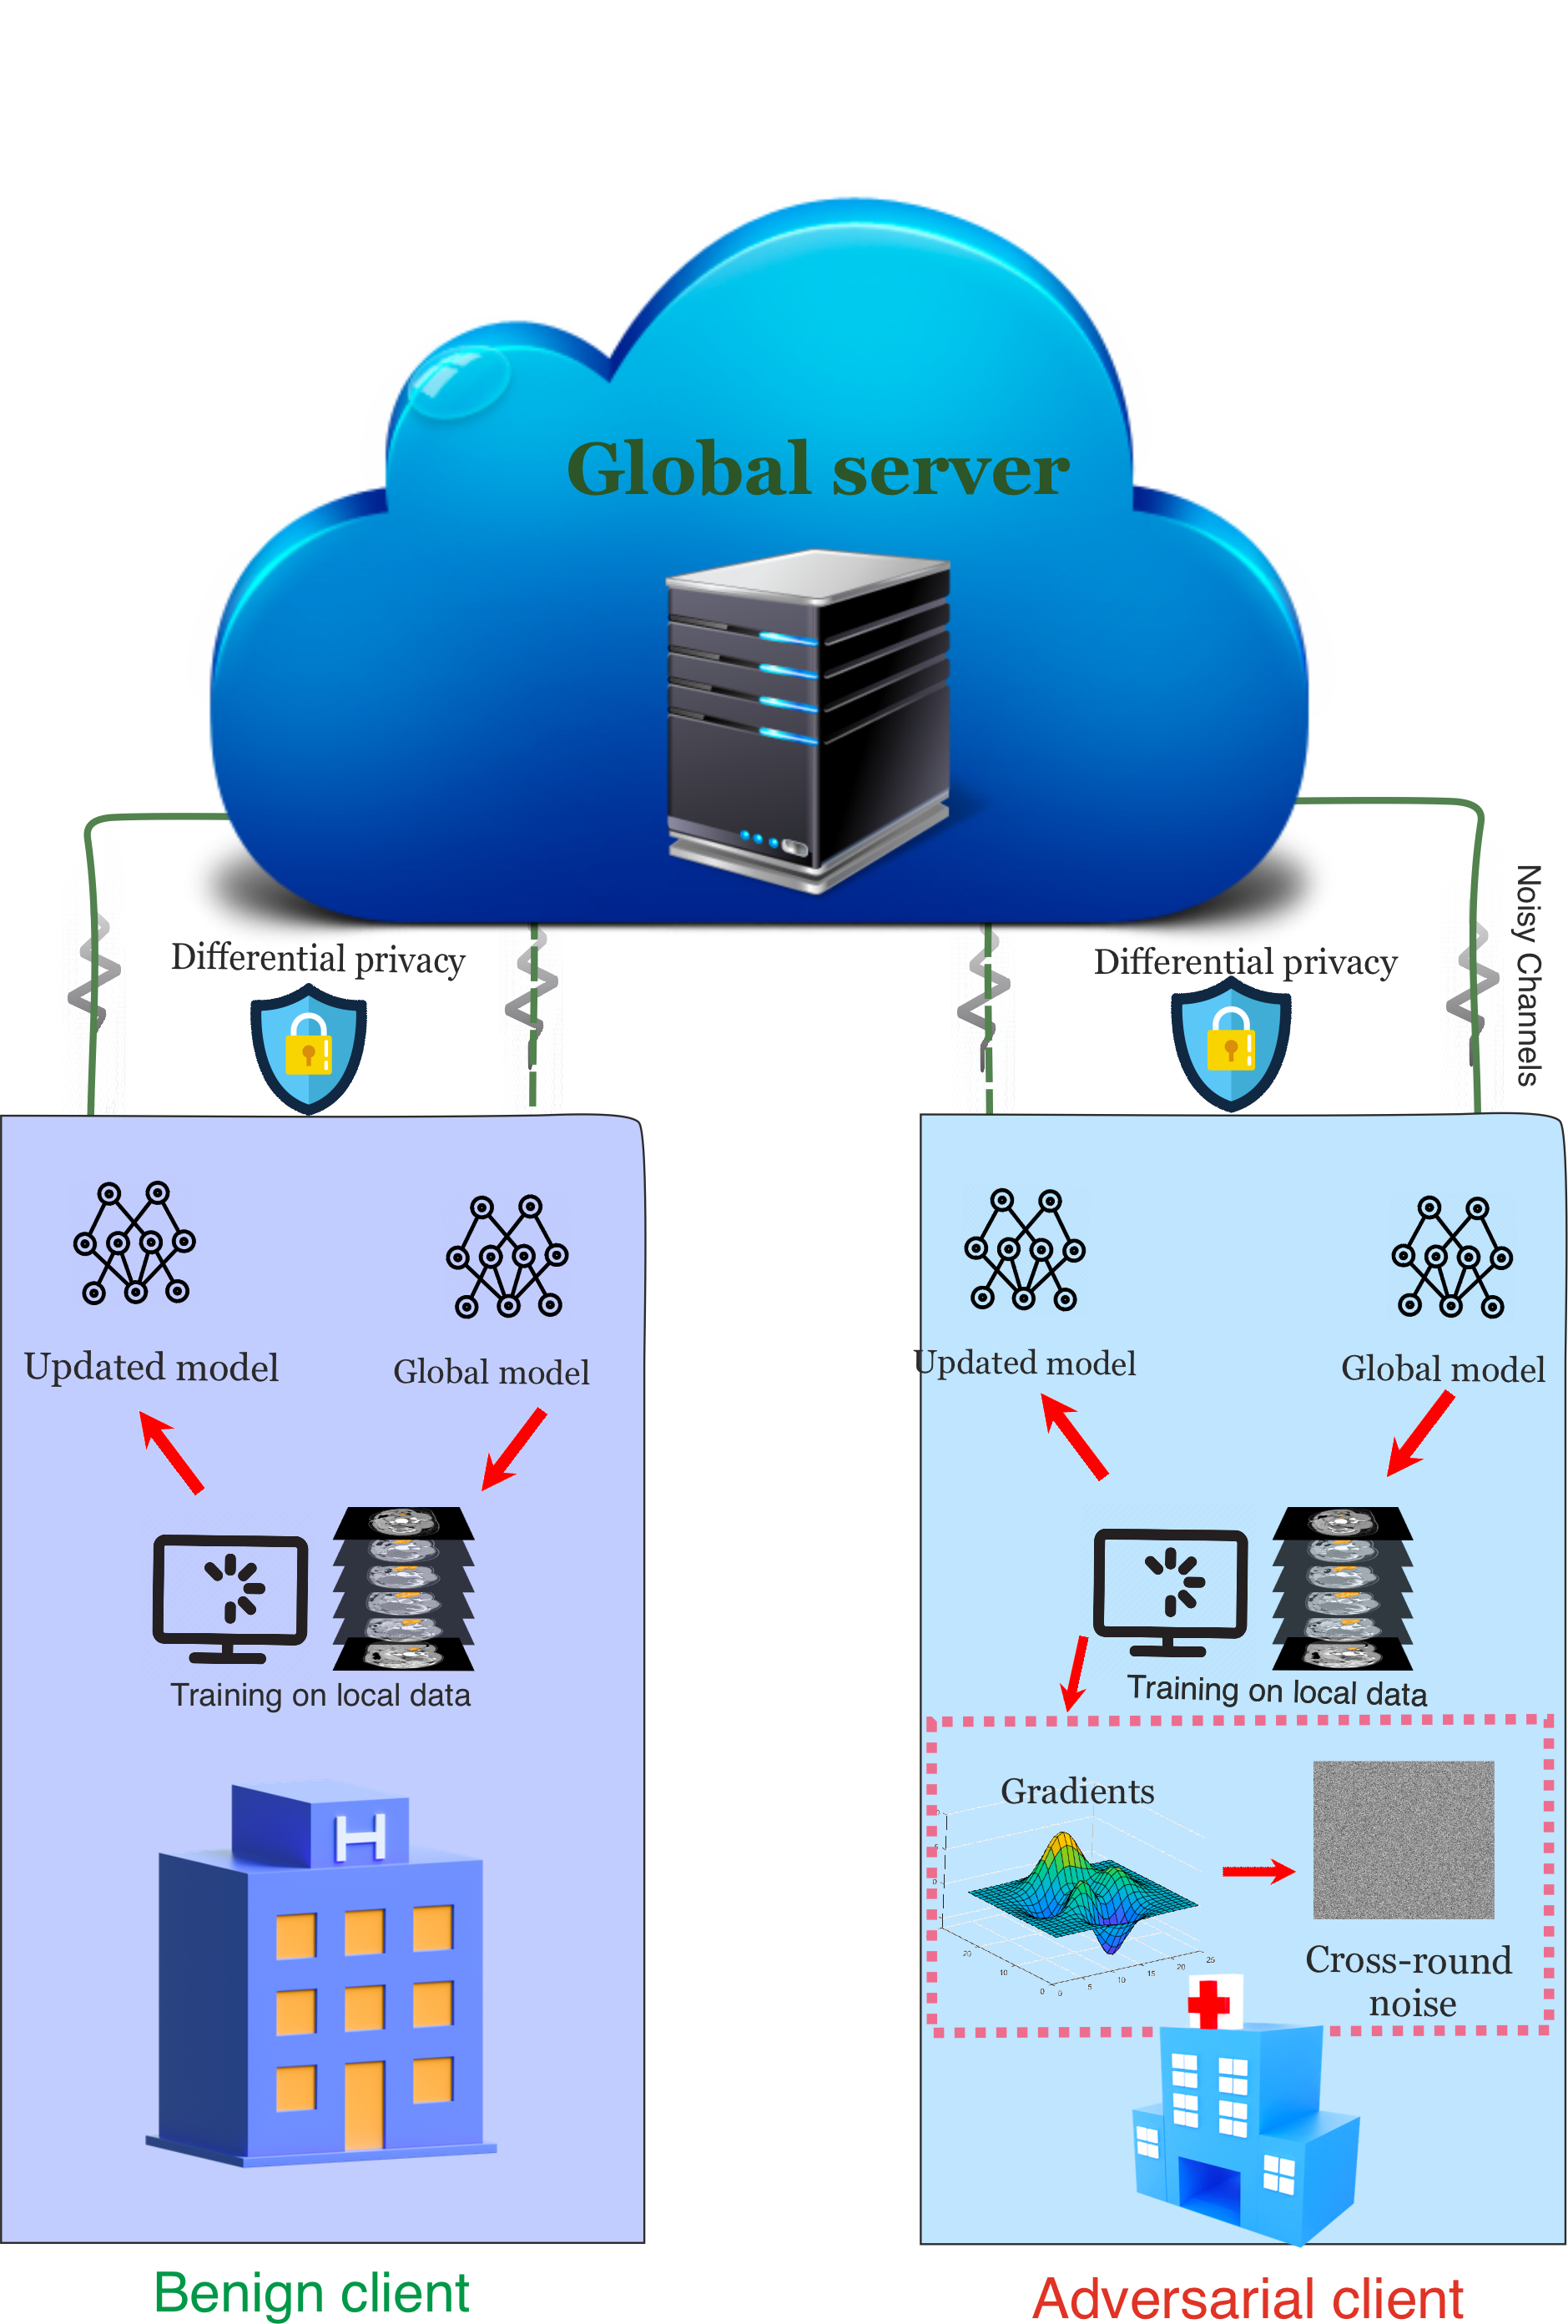
\includegraphics[width=0.50\textwidth]{Adversarialattacks.png}
 \caption{A schema of our method, at each FL round, the adversary transforms the gradients into cross-round noise, while acting as a benign client and not tampering the training process}
 \label{fig:pgd-atta-comparison}
\end{figure}

\subsection{Attack models}
Numerous adversarial attacks have been proposed by the literature in order to fool deep neural networks and produce false predictions. Adversarial attacks work through injecting a guided imperceptible noise that fools the trained deep learning model. Popular methods are  FGSM, PGD, and BIM attacks which will be discussed.

\textbf{FGSM:} Fast Gradient Sign Method (FGSM) \cite{szegedy2013intriguing}is a fast yet effective method which produces adversary image with one step of calculation. Assuming input $x$ and its corresponding target $t$, FGSM calculates gradient of $x$ w.r.t the loss function ${\partial \mathcal{L}}/ \partial {x}$.

\begin{equation}
\label{eqt:fgsm}
    \bm{\hat{x}} = \bm{x} + \epsilon \cdot sgn\big(\nabla_{\bm{x}}{\mathcal{L}}(g(\bm{x};w)\big)
\end{equation}

where epsilon $\epsilon$ is a hyper-parameter which determines adversarial noise level. $g(\bm{x};\bm{w})$ is the output of neural network with respect to the input $x$ and parameter set $w$. $sgn(.)$ is the sign function. The result of sign function goes through a clipping function to impose a maximum bound in change to the perturbation $\epsilon \cdot sgn\big(\nabla_{\bm{x}}{\mathcal{L}}(g(\bm{x};\bm{w})\big)\in [-1,1]$.

\textbf{BIM:}  Basic Iterative Method (BIM) is an extension of the FGSM method, By Kurakin et al.\cite{kurakin2018adversarial} repeatedly do the process in FGSM, using a small step-size and $\bm{\hat{x}^{1}} = \bm{x}$. BIM is stronger than FGSM and requires smaller perturbations.

\textbf{PGD:} Madry et al. \cite{madry2017towards}proposed their own version of the BIM attack. In Projected Gradient Descent (PGD) \cite{madry2018towards}
the attack starts with a uniform random initialization. The update formula for PGD attack can be written as: 
\begin{equation}
\label{eqt:pgd}
    \bm{\hat{x}}^{t+1}=\Pi_{P_\epsilon(\bm{x})} \Big( \bm{\hat{x}}^t + \alpha \cdot sgn\big(\nabla_{\bm{x}}{\mathcal{L}}(g(\bm{\hat{x}}^t;\bm{w}),t)\big)\Big)
\end{equation}
Where $\bm{\hat{x}}^{k}$ is the perturbed data in $k$-th iteration, and $P_\epsilon(\bm{x})$ is the projected gradient descent function, which is done by first finding sign values, and then projecting the result to a small neighborhoud of the input ${x}$. This possible parameter spaces determines the set PGD attack samples that an adverdsary can use. PGD is one of the strongest attacks and is a universal first-order adversarial method. Technically, aside from formulazing the problem as projected gradient, PGD is similar to BIM but with random small initialization. We report results with PGD. With same number of iterations, BIM had the same results, or the difference was negligilbe.
	
% \subsection{Optional}
% blackbox/wihtebox
\section{Enhanced adversarial attack }
\label{sec:ourattack}
In this section we introduce our method to enhance the existing adversarial attacks in an FL setting.

\subsection{Threat model}


% \begin{algorithm}[th]
%  \caption{Adversarial Training with Transferable Adversarial Examples (ATTA)}\label{alg:atta}
%  \begin{algorithmic}[1]
%  \State \textbf{Input}: Padded training dataset $D_{nat}$, model $f_\theta$, attack algorithm $\mathcal{A}$, perturbation bound $\epsilon$, the number of epochs to reset perturbation $reset$
%  \State Initialize $\theta$
%  \State Initialize $D$ by cloning $D_{nat}$
%  \For{$epoch = 1 \cdots N$}
%  \For{$x_{nat},y$ in $D_{nat}$ and corresponding $x \in D$}
%  \If {$epoch\ \%\ reset\ =\ 0$}
%  \State $\beta \gets$ a small random perturbation
%  \State $x \gets x_{nat} + \beta$
%  \EndIf
%  \State Store the transformation $T_{aug}$ for the inverse augmentation:
%  \State $x_{aug}, x_{nat, aug}, T_{aug} \gets \dataaug(x, x_{adv})$
%  \State $x^* \gets \mathcal{A}(f_{\theta}, x_{nat, aug}, y, x_{aug}, \epsilon)$
%  \State $\theta \gets \theta - \nabla_{f_{\theta}} \frac{\partial \mathcal{L}(f_\theta, x^*, y)}{\partial \theta}$
%  \State $x \gets \inverseaug(x, x^*, T_{aug})$
%  \EndFor
%  \EndFor
%  \end{algorithmic}

% \end{algorithm}




We consider a scenario in which one FL participant is malicious or is controlled by a hostile adversary. The adversary tries to fool the global model by generating images similar to its real data.
We assume that the central server is honest and trusted.\\\textbf{Goal of adversary:}
The adversary's Goal is to manipulate the global model so that the global model has a higher classification error.  \\
\textbf{Knowledge of adversary:}
In a realistic scenario, the malicious party only can see its own data $D_{i}$, and knows the DNN architecture and the global model weights that it receives each round. \\
\textbf{Capability of adversary:}
No special privilege or Capability is assumed for the adversary. Similar to other clients, the adversary has control over its own training procedure and data, and it can not manipulate other clients' data or the general learning process. (e.g., local computations, communication with central server and aggregation process, DNN architecture, and optimization functions). It can interact with the model, query the outputs, and calculate the gradients. The adversary doesn't use the training data.




\subsection{Cross-round noise}



Adversarial examples being developed in the inference time, the adversary might not have the necessary computing power as they have during the training time. Also, sometimes inference is being done on third-party applications on edge devices where they don't have GPUs.
This might be crucial for the adversary, that it can prepare the attack samples with less computations. Iterative methods, such as PGD, require too much computational power to develop the examples. even more than normal training itself. \cite{zhang2019you} The problem could be worse for high-resolution or whole-slide images.
Also, PGD needs the target and surrogate to be highly similar to ensure transferability. However, models being noisy causes high inter-client variability, as a protection measure.

% Federetaed environemtn can introduce new surfaces to enhance adversarial transferability.  Gather more information about other clients by utilizing  global model upates.\cite{lyu2020threats}


% \begin{figure}[htbp!]
%  \centering
%  \includegraphics[width=0.10\textwidth]{Adversarial0attacks-7.eps}
%  \caption{Traditional adversarial training (PGD-$k$) (a) and ATTA-$k$ (b). $C$ is the connection function which improves the transferability between epochs.}
%  \label{fig:pgd-atta-comparison}
% \end{figure}
Incorporating prior knowledge already available from the global model, the attack can be initialized from a proper baseline so the computation might be reduced. Also, it might diminish the bias and lead to a broader estimation of other clients.



We introduce an intermediary noise tensor we call \textit{Cross-round noise} which extracts features from received global and is calculated alongside local epochs. The noise gets updated and passed to the next FL round. 
We use a function for the adversary to produce a noise based on ${L}_{2}$ regularized gradients at each FL training round. Then in the test phase, we use the noise to initialize the values for adversarial attack algorithms. 



\begin{algorithm}[t!]
\caption{Training procedure}
\label{alg:NbAFL}
\LinesNumbered
\KwData{$T$, $\beta$, ${w}^{(0)}$, $\mu$, $\epsilon$ and $\delta$}
{Initializing parameters: $t = 1$ and ${w}^{(0)}_{i} = {w}^{(0)}$ and ${{\mathcal{\delta}}^{(t)}=0}$} $\forall i,t$\\
\While {$t \le T$}
{
\textbf{Local training:}\\
\While {$\mathcal C_i\in \{\mathcal C_1, \mathcal C_2, \ldots,\mathcal C_{N}\}$}
{
Clients update their models ${w}^{(t)}_{i}$ as\\
% \quad\quad ${w}^{(t)}_{i}=\arg\min\limits_{{w}_{i}}{\left(F_{i}({w}_{i})+\frac{\mu}{2}\Vert {w}_{i}-
\quad${w}^{(t)}_{i}=\arg\min\limits_{{w}_{i}}{\left(\mathcal{L}_{i}({w}_{i})\right)}$\\
Clients clip parameters ${w}^{(t)}_{i} = {w}^{(t)}_{i}/\max\left(1,\frac{\Vert{w}^{(t)}_{i}\Vert}{C}\right)$\\
Clients add Gaussian noise\\ $\widetilde{{w}}^{(t)}_{i}={w}^{(t)}_{i}+{n}^{(t)}_{i}$\\
}
\textbf{Global update:}\\
Global server individual models ${w}^{(t)}$ as\\
\quad\quad ${w}^{(t)} = \sum\limits_{i=1}^{N}{p_{i}\widetilde{{w}}^{(t)}_{i}}$\\
Global server adds Gaussian noise \\
\quad\quad$\widetilde{{w}_{i}}^{(t)}={w}^{(t)}+{n}_{\text i}^{(t)}$\\
\If{$t \ge \beta$}
    {
% \textbf{Adversairal client:}\\
  \textbf{Adversarial client} $\mathcal C_{m},   \mathcal X \in \mathcal D_m:$
  % ,  {\mathcal{\delta}^{(\beta)}=0,$:}\\
% \quad\quad
\\Adversary performs gradient regularization \\
\quad{${{\nabla_{\mathcal{X}}\mathcal{\hat{L}}\gets \nabla_{\mathcal{X}}\mathcal{L}(\mathcal {\delta}^{(t-1)},\widetilde{{w}_{m}}^{(t)}})}$}\\
% ${\mathcal{\delta}}^{(t)}\gets \epsilon . sgn(\nabla_{\mathcal{X}}\mathcal{\hat{L}}(\mathcal {\delta}^{(t-1)},\mathcal{X},\widetilde{{w}_{m}}^{(t)})$
% \quad\quad${{\mathcal{\delta}}^{(t)}\gets \epsilon . sgn(\nabla_{\mathcal{X}}\mathcal{\hat{L}}(\mathcal {\delta}^{(t-1)},\widetilde{{w}_{m}}^{(t)}}))$
\\Adversary projects the gradient \\

\quad$\mathcal{\delta}^{(t)}\gets \Pi_{P_\epsilon(\bm{0})}(\nabla_{\mathcal{X}}\mathcal{\hat{L})}$
}
% Test the received parameters $\widetilde{\mathbf{w_{i}}}^{(t)}$ using local dataset\\
% 
\\$t\leftarrow t + 1$}
% #2ndPart#########################
% #2nd Part#########################
% #2nd Part#########################
% #2nd Part#########################
% #2nd Part#########################
% #2nd Part#########################
% #2nd Part#########################
% #2nd Part#########################
% #2nd Part#########################}
% \textbf{Adversarial attack process:}\\
% % {Initialization: $\mathcal$ and ${w}^{(0)}_{i} = {w}^{(0)}$} 
% {\While \{$\mathcal C_i\in \{\mathcal C_1, \mathcal C_2, \ldots,\mathcal C_{N}\}$}
% { 
% Update the local parameters ${w}^{(t)}_{i}$ as\\
% % \quad\quad ${w}^{(t)}_{i}=\arg\min\limits_{{w}_{i}}{\left(F_{i}({w}_{i})+\frac{\mu}{2}\Vert {w}_{i}-}
% }
% % Test the receivedparameters $\widetilde{\mathbf{w_{i}}}^{(t)}$ using local dataset\\
% $t\leftarrow t + 1$}}}
% % \KwResult{$\widetilde{{w}}^{(T)},{\mathbf{\mathcal{{\delta}}}^{T}}$}}
\KwResult{$\widetilde{{w}_{i}}^{(T)},{\mathbf{\mathcal{{\delta}}}^{T}}$}
\end{algorithm}

\subsubsection{Gradient calculation}


The noise is calculated by the gradients of model at each round. The adversary uses the loss:

% \begin{equation}
% \label{eqt:loss}
% L(f_{r}({x}_{adv},f_{r}{(x))})
% \end{equation}


\begin{equation}
\label{eqt:loss1}
 \nabla_{\bm{x}}{\mathcal{L}}(g(\bm{x+\delta}^{(t)};\bm{w^{(t)}}),g(\bm{x};\bm{w^{(t)}}))
\end{equation}
% \hl{BIM/ PGD ro yejuri joda kon}
To update the stored values for the noise. In which $g(.;\theta^{t})$ refers to received global model in communication round $t$.  The adversary iteratively updates the noise by maximizing the loss between the model output for the noisy and the clean test data. 
% Here we assumed that the adversary does not have access to the labels. So the true labels are not used for the loss function. 
% \hl{mituni bahs koni chera in behtar az ine ke loss ro nesbat be label hesab konim}. 
The global model parameters change for the test dataset being the same in each round. 
\cite{zhang2019theoretically}
Saving noise could be started after an arbitrary number of rounds is passed, say, $\beta$ and be calculated alongside local training with similar epochs. In this paper, we consider initializing from the last 10 and last 5 rounds. Calling them CRN10 and CRN5 respectively.
% This process can also be done for several iterations, depending on the value of $\epsilon$.
% \hl{$\beta$ ro  .iar too bahs}
\\\subsubsection{$L_{2}$ regularization}

Transferring gradient information between models might lead to drastic parameter change.\cite{zhang2019theoretically,pan2019improving,dettmers20158}. Unlike some methods which manually reset the gradients, so they lose information \cite{zheng2020efficient}, we regularize the change in CRN by subtracting the mean value in each channel of the input noise. We apply a function for $L_{2}$ regularization the gradients.
\begin{equation}
    \nabla_{x_{i}}\mathcal{\hat{L}} = \nabla_{x_{i}}\mathcal{{L}} -  \frac{1}{M} \sum\limits_{j=1}^{M}{\nabla_{x}_{_{i,j}}} \mathcal{{L}}
\end{equation}
The resulting value is channel-wise regularized loss, and $i$ indicates index of channel, and $j$ refers to individual pixels. This results in a smaller $L_{2}$ norm of gradient values, which is a proven measure against explosion or outlier gradients. \cite{pascanu2013difficulty}\cite{kim2016accurate} . 
\\Then it goes through projection procedure, which the final values are $L_\infty$ bounded around zero, with a small value $\epsilon$. 
% To ensure the noise stays sufficiently small 


\subsection{Inference phase attack}
Attacks are performed after training is done. FGSM and BIM use zero initialization, and PGD uses random initialization, then they compute the adversarial example according to Equations \ref{eqt:fgsm} and \ref{eqt:pgd}.\\
We use the cross-round noise added to the input test data as an initial point for these methods, \\



showing that they can improve substantially.\\ Adversarial examples can be computed even with one step of computation, and non-iterative models like FGSM can be strong enough to outperform PGD with random initialization.\\
These iterative algorithms put lots of loads since the projected gradient descent is very expensive to compute. \cite{shafahi2019adversarial}
It is possible that models are integrated into another environment like PACS or software. Training these models is time-consuming and might be a burden.




 
\section{Experiment}
\textbf{Dataset} Our experiments used two publicly available data sources, the Tongji hospital dataset\cite{yang2020covid} and Brazil's SARS-CoV-2 dataset\cite{soares2020sars} Tongji dataset consists of 349 chest CT-scans of COVID-19 positive and 397 scans of healthy subjects, all low-resolution CT modalities. Brazil's SARS-CoV-2 dataset consists of 2482 samples, 1252 scans of COVID-19-infected patients, and 1230 healthy subjects collected from multiple hospitals in Sao Paulo, Brazil. The datasets are approved by the corresponding ethical committees of each hospital, Public Hospital of Sao Paulo (HSPM), and Tongji Hospital in Wuhan, China. Train and test sets were obtained randomly from the aggregated datasets. Table \ref{table_datadist}, shows data distribution.


\begin{table}[h!]
\centering
\setlength{\tabcolsep}{6pt}
\renewcommand\arraystretch{1.22}
\caption{ \small Data distribution}
\begin{tabular}{| *{5}{c|} }
\hline
Class  & Dataset & Samples & Train & Test
\\   \hline  
\multirow{2}{3em}{COVID}     &Brazil&1252&\multirow{2}{2em}{1451}  &\multirow{2}{2em}{150}  \\
&Tongji&349&&  \\
\hline
\multirow{2}{6em}{Non-COVID}     &Brazil&1230&\multirow{2}{2em}{1477}  &\multirow{2}{2em}{150}  \\
&Tongji&397&&  \\
\hline
\end{tabular}
\label{table_datadist} 
\end{table}


\textbf{Preprocessing}
Images were selected as 2D slices in greyscale. Preprocessing included randomly cropping between 0.5 to full size, random horizontal flipping, and intensity normalization. CT-slices were all resized to 224$\times$224 pixels with interpolation. Figure \ref{fig:samplesCTs} shows samples of processed images.
% \quickthings{This looks like you have a bias in your dataset. You should select the normals and abnormals at comparable level in the thorax. All covid are now lower in the body then the non-covid ones.}
% \maybelater{I have changed the picture, hope it's okay now}
\begin{figure}[h!]
 \centering
 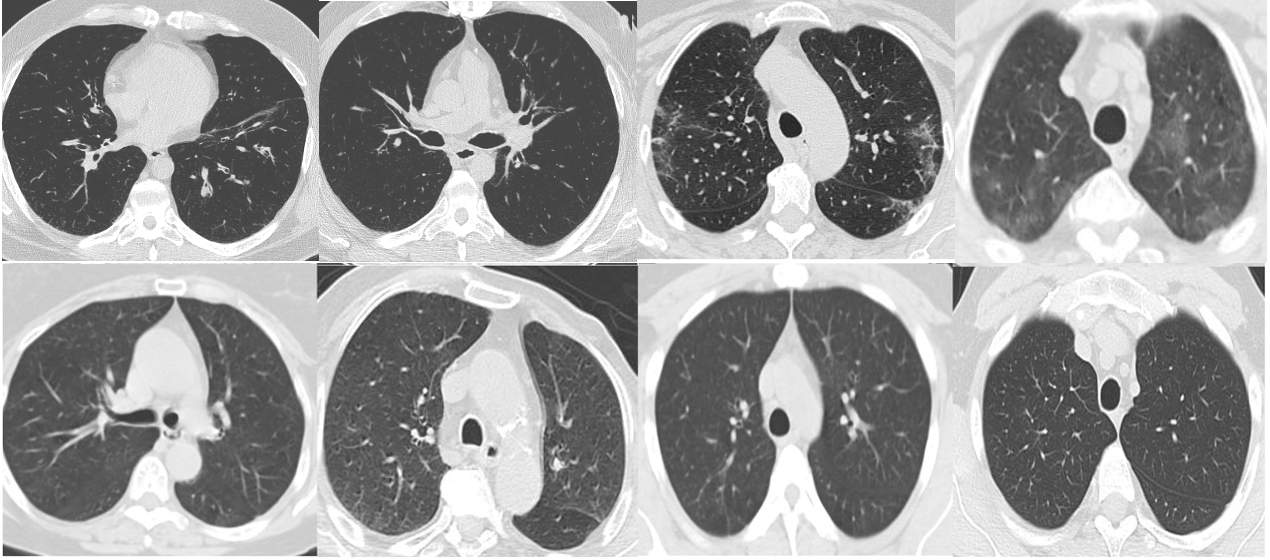
\includegraphics[width=0.45\textwidth]{covidexamples3.png}
 \caption{Sample CT slices of COVID-19 images (top row) and Non-COVID images (bottom row)}
 \label{fig:samplesCTs}
\end{figure}


% normalize = transforms.Normalize(mean=[0,0,0], std=[1,1,1])
% train_transformer = transforms.Compose([
%     transforms.Resize(256),
%     transforms.RandomResizedCrop(224, scale=(0.5, 1.0)),
%     transforms.RandomHorizontalFlip(),
%     transforms.ToTensor(),
%     normalize
% ])

\textbf{Training}
ResNet-18 is used as the backbone deep learning model. ResNet-18 comprises one initial block cascaded to four middle blocks. The initial block is made of convolutional,  batch normalization, ReLU, and pooling layers. Middle blocks have the same layers, connected with straight and skip connections. The model is pre-trained on ImageNet dataset \cite{he2016deep} with a CrossEntropy loss function and learning rate of $0.05$. 
Each federated round consisted of 20 internal epochs for each client and batches of 16 samples in each iteration. For models which use minibatch training, like STWT and FedSGD, a subset of clients is randomly selected. Similar to training, test data was split into mini-batches, and the results were averaged across batches. We performed training with various participating clients and federated rounds to evaluate their effect on final performance. Models were also trained in a centralized, non-federated setting to build a comparison baseline. Figure \ref{fig:distributionsite} shows the data distribution among clients.

\begin{figure}[h!]
 \centering
 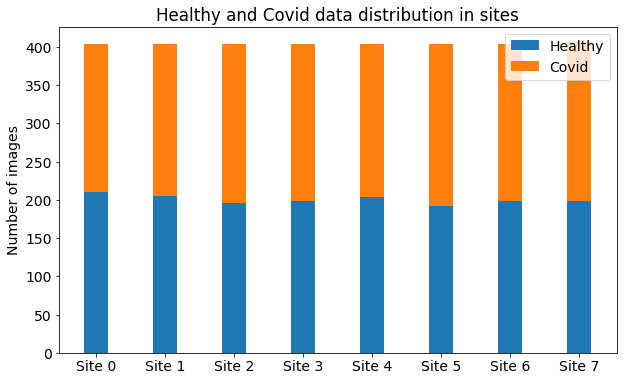
\includegraphics[width=0.7\textwidth]{output.png}
 \caption{Data distribution of each client in the simulated federated setting}
 \label{fig:distributionsite}
\end{figure}
% \abs{Healthy COVID data distirbution per site}

\textbf{Evaluation} 
Standard classification metrics, accuracy, recall, precision, and F1 score, were used as our evaluation criteria. We also evaluated the level of communication, the amount of transferred data in each algorithm, and the computational complexity of the models. 
\label{sec:experiment}


\section{Results}


% In order to evaluate and compare federated learnign models 
% Specificity  and  sensitivity  are  the  abilities  of  a  model  that how correctly the model identifies a subject with disease and without a disease. 
% In our case, it is critical to detect a COVID-19 patient as missing a COVID-19 patient can have disastrous consequences.   

% A medical diagnosis based system needs to have high sensitiv- ity and recall. 
Here, the result for the setting with 10 participating clients and a maximum of 10 rounds is presented. The results are average performance among clients for all the federated rounds. Table \ref{best_performance} shows the results.
% \quickthings{Why comparison of FedAVG and CWT?}\maybelater{I removed the sentence}
% The average score in each state could be a way to reach them—the average scores in F1, FedSGD, CWT, and SWT. 
% The FedSGD models have been used are
% The results for CDS are also included as a benchmark ground truth.

% \quickthings{Put CDS at the top, keep same order as in the materials and methods. Consistency!}
% \maybelater{Fixed!}

\begin{table}[h!]
\centering
\setlength{\tabcolsep}{5.5pt}
\renewcommand\arraystretch{1.12}
\caption{ \small Comparison of FL algorithms on classification of COVID-19 data for 10 clients, averaged performance in all the 10 rounds.}
\begin{tabular}{| *{5}{c|} }
\hline
Method & Accuracy & Recall & Precision & F1 score
\\
  \hline
  

CDS
 &87.75\%&89.57\% &87.93\% & 87.19\%  
\\   \hline  
FedAVG
 & 66.72\% &70.02\% &43.80\% & 51.7\%\\ 
 \hline  
FedSGD
 &65.17\% &68.24\%&43.86\%& 47.75\%  
 
 \\
 \hline  
CWT
 &87.75\%&89.00\%& 88.67\%&87.52\%\\
 
   \hline
 

SWT
 & 64.60\% &74.33\% & 65.55\% &59.66\% \\
    
\hline 
STWT
 & 84.21\% &84.09\%&83.33\% & 81.71\%  \\



\hline
\end{tabular}
\label{best_performance} 
\end{table}


\textbf{Assesing the impact of training rounds} To evaluate the effect of number of rounds, models with 3, 5, 10 and 15 rounds were tested. The test results are shown for both centralized and FL  algorithms. Table \ref{number_of_rounds} shows the results of our experiment. The increasing number of rounds correlates with higher accuracy of the global model.
% \quickthings{Same with table III, put at the top.}

% \maybelater{done}

% \begin{table}[h!]
% \centering
% \setlength{\tabcolsep}{5.5pt}
% \renewcommand\arraystretch{1.12}
% \caption{ \small Effect number of rounds on models' accuracy}
% \begin{tabular}{| *{5}{c|} }
% \hline
% Method & 3 rounds & 5 rounds & 10 rounds & 15 rounds 
% \\   \hline  
% FedAVG
%  & 66.28\% &77.24\% & 86.63\% & 94.03\%\\

%  \hline
%  FedSGD
%  &  53.77\% & 70.55\% &90.04\% & 92.75\%\\
% \hline  
% % SWT
% %  &  85.34\% & 97.24\% &93.63\% & 98.74\%\\
% % \hline  
% CWT
%  &  96.02\% & \textbf{98.44\%} &\textbf{99.29\%} & 99.86\%\\

% % \hline  
% % CDS
% %  to be completed!


% \hline  
% STWT
%  &  \textbf{96.59\%} & 97.72\% &99.57\% & \textbf{100.00\%}\\

 
%  \hline
% CDS
%  &92.03\% &88.34\% & 98.01\% & 100.00\% \\
%  \hline
% \end{tabular}
% \label{number_of_rounds} 
% \end{table}


\begin{table}[h!]
\centering
\setlength{\tabcolsep}{3.5pt}
\renewcommand\arraystretch{1.12}
\caption{ \small Effect number of rounds on accuracy of FL algorithms for 10 clients, 20 internal epochs.}
\begin{tabular}{| *{5}{c|} }

% \begin{tabular}{| {c|}{c|}{c|}{c|}{c|}{c|}{c|}{c|}{c|} |}
\hline
% Method & \multicolumn{2}{c}{3 rounds} & \multicolumn{2}{c}{5 rounds} &\multicolumn{2}{c}{10 rounds} &\multicolumn{2}{c}{15 rounds} 

Method & 3 rounds & 5 rounds & 10 rounds & 15 rounds
%  & M &SD & M &SD& M &SD& M &SD 
\\
 \hline
CDS
 &85.06\% &81.56\% & 91.06\% & 91.04\% 
\\
\hline
FedAVG
 & 56.05\%  &63.78\%&69.64\%&70.73\% \\

 \hline
 FedSGD
 &  50.88\% & 55.9\% &75.59\% & 76.94\%\\
% \hline  
% SWT
%  &  85.34\% & 97.24\% &93.63\% & 98.74\%\\
\hline  
CWT
 &  80.77\% & \textbf{89.78\%} &\textbf{91.27\%}& \textbf{93.56\%}\\

% \hline  
% CDS
%  to be comp,';leted!


\hline  
STWT
 &  \textbf{90.73\%} & 83.97\% &89.44\% & 93.01\%\\

 
  \hline

\end{tabular}
\label{number_of_rounds} 
\end{table}
\quickthings{Shouldn't this column have the same results as table II for accuracy?}

\peter{Table III and Table II do not represent the same thing. Table II is average performance in all 10 rounds, is to give an overall impression of accuracy, and table III is the final result in the end of the 5th, 10th , 15th rounds.  Added  to the table caption.
}
% \maybelater{The results are for max, maybe you want to add average results later?}
% \maybelater{Having the same thing (acc) for other metrics such as F1, prevciison recall etc}

\textbf{Assessing the influence of client participation}
To evaluate the number of clients on the FL network, we examined scenarios with 3,5, and 8 participating clients. We trained each of the clients in 20 internal epochs. The number of Federated rounds for all the algorithms (except SWT) was 10.
The average test results are shown in the Figure \ref{fig:data distribution}. \quickthings{Why not a column for 10 clients here?}
\maybelater{ 10 clients are shown in table three , third column. Added 10 clients here as well}

% \begin{table}[h!]
% \centering
% \setlength{\tabcolsep}{7pt}
% \renewcommand\arraystretch{1.22}
% \caption{ \small Effect number of clients on accuracy of FL algorithms, 10 rounds, 20 internal epochs.}
% \begin{tabular}{| *{9}{c|} }
% \hline
% Method & 3 clients & 5 clients & 8 clients 
% \\   \hline  
% FedAVG
%  & 79.52\% &70.73\% & 63.98\% \\

% \hline  
% FedSGD
%  & 78.02\% &75.59\% &69.76\%  \\
% \hline  
% CWT
%  &  89.90\% & \textbf{91.27\%} &\textbf{88.98\%} \\
%  \hline
% STWT
%  &  \textbf{90.93\%} & 89.44\% &84.57\% \\
%  \hline  
% SWT
%  & 55.80\% &69.19\% & 68.81\%\\




% \hline  
% CDS
%  to be completed!

% \hline  

% \end{tabular}
% \label{effect_num_clients} 
% \end{table}


\begin{figure}[h!]
 \centering
 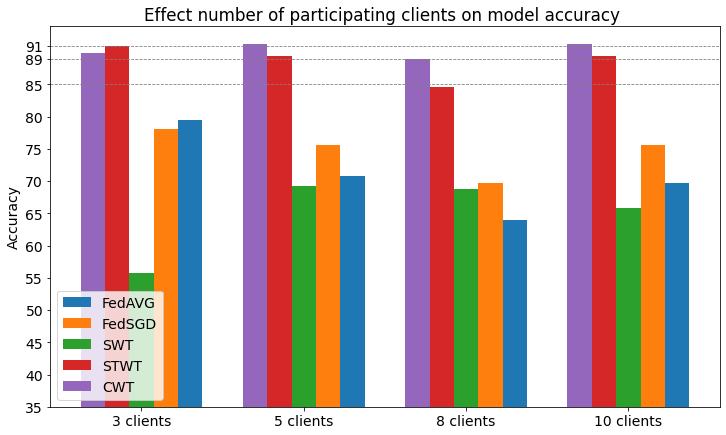
\includegraphics[width=0.7\textwidth]{download.png}
 \caption{Accuracy of FL algorithms with differrent number of clients. }
 \label{fig:data distribution}
\end{figure}


% \maybelater{Maybe taking MAX is better instead of latest epoch?}

 
\begin{figure}[h!]
 \centering
 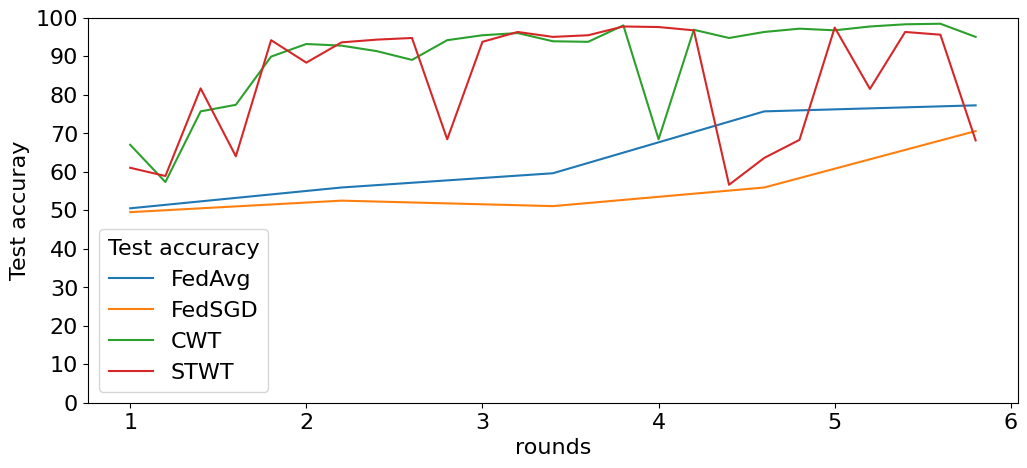
\includegraphics[width=0.7\textwidth]{cyclic.png}
 \caption{Test accuracy as a function of passing rounds}
 \label{seq-vs-noseq}
\end{figure}
% \maybelater{Best accuracy vs Average accuracy for showing that SWTW works bad in average but well in best accuracy}
% \abs{Adding a graph showing arrows for gradient updates}
% \maybelater{Maybe adding 10 clients?}
% \maybelater{8 ta client, 4 FL rounds
% 20 each client for CWT plot . and also 8 ta client, 4 FL round 20 each client for FedSGD and FedAVG}
% \subsection{Other graphs}

\begin{table}[h!]
\label{computation time}
\centering
\setlength{\tabcolsep}{7pt}
\renewcommand\arraystretch{1.22}
\caption{ \small Computation time (seconds) for FL algorithms for standardized setting}
\begin{tabular}{| *{9}{c|} }
\hline
Method & 3 clients & 5 clients & 8 clients  & 10 clients
\\   \hline  
FedAVG
 & 8934 sec&8975 sec  & 9002 sec & 9030 sec\\

\hline  
FedSGD
 & 8810 sec &8853 sec& 9013 sec & 9052 sec \\
\hline  
CWT
 &  5119 sec& 5450 sec&5383 sec & 5556 sec\\
 \hline
STWT &
2805 sec&  5243 sec& 6101 sec & 6129 sec\\
 \hline  
SWT
 & \textbf{543 sec} &\textbf{547 sec} & \textbf{589 sec } & \textbf{618 sec}\\



% \hline  
% CDS
%  to be completed!

\hline  

\end{tabular}
\label{computation_time} 
\end{table}


Communication can also be a bottleneck in this setting. In methods like federated averaging, the lower bounds for total communicated data are proportional to $\sim$
${2NT}$
where the total rounds are represented by T and the count of involved clients is denoted by N. In CWT, this lower bound is  $\sim$ ${NT}$. In our setting, we use a ResNet 101 model. We calculated the overall transferred data for the different number of rounds. As expected, the experiments show that when clients are selected randomly, the communication time tends to be shorter compared to scenarios involving participation from all clients. Moreover, our analysis of computational costs indicates that models that do not rely on sequential processing generally demand higher computational resources compared to their sequential counterparts. The detailed results for computational and communication evaluations can be found in Table \ref{computation_time} and Table \ref{transferredData}, respectively.
\quickthings{Again, why only this comparison is relevant enough to put into the text?}
\maybelater{Here fedavg, and fedsgd are the same family, (non sequential), and CWT are the other family (sequential)., Changed the phrasing from CWT/FedAVG to seq/non-seq, hope it's okay this time.}

\begin{table}[h!]
\centering
\label{Transferred data}
\setlength{\tabcolsep}{5.5pt}
\renewcommand\arraystretch{1.12}
\caption{ \small Comparison of total transferred data in a normalized setting (GB)}
\begin{tabular}{| *{5}{c|} }
\hline
Method & 3 rounds & 5 rounds & 10 rounds & 15 rounds 
\\   \hline  
FedAVG
 & 1.371 &2.286 & 4.571 & 6.857\\

 \hline
 FedSGD
 &  0.823 & 1.371 &2.743 & 4.114\\
\hline  
% SWT
%  &  85.34\% & 97.24\% &93.63\% & 98.74\%\\
% \hline  
CWT
 &  0.686 & 1.143 &2.286 & 3.428\\

% \hline  
% CDS
%  to be completed!


\hline  
STWT &
  0.411 & 0.686 &1.371 & 2.057\\

 

 \hline
\end{tabular}
\label{transferredData} 
\end{table}





% \maybelater{Momkene computational complexity ro beshe ba order nevesht? peida kon settingesh ro}
% \maybelater{Graphs showing results}
% \maybelater{Comparison of FL models}
% \maybelater{Loss/round}
% \abs{definition of precision and recall}


\label{sec:results}



% \newpage


\section{Discussion}
\label{sec:discussion}

% Local training had near random accuracy, but in all the experiments, the performance results were improved. 
% Considering low number of samples for individual clients, a training process limited to few clients results in near random classification accuracy. 
% Local models can have low performance due to limited datasets.
% Also,, ImageNet pre-training had a speed-up effect on our model performance.

% \textbf{Fundamental groups of FL}

% \textbf{how many groups}
% \textbf{how can we group them, name different ways}
% \textbf{effect number of data}


% Paragraph 1: This paragraph provides a “big picture” perspective for readers to remind them of the importance of your study.

% \textbf{overall results}
% 
Our results show that FL has comparable performance to centralized data sharing, with the advantage of keeping data private. With large volumes of data and after high number of rounds, centralized data sharing and cyclic weight transfer have the highest accuracy. 


Sequential models are susceptible to catastrophic forgetting, where a global model performs well on the latest client it has seen while having poor performance in other clients.\quickthings{cryptic sentence}\maybelater{I have paraphrised the sentence}
Conversely, in algorithms like FedAvg and FedSGD, the models are averaged asynchronously after all the clients have finished their training. So the trajectory is smoother and overall improving with more communication rounds. As shown in Figure \ref{seq-vs-noseq}, local test results can have a high variance when passing through clients sequentially, indicating the catastrophic forgetting effect.

Models like FedAvg, and FedSGD, in which all the clients have identical copies of one global model, are slower and more challenging to converge compared to sequential models like CWT and STWT. Also, FedAvG and FedSGD require more training resources due to active server participation, resulting in more computation and network consumption. Stochastic client selection is an efficient way of training. Stochastic models save significant time and resources while having similar performance to full client participation. Overall, CWT and STWT have best results in terms of model accuracy and computation times. These findings could be practical in further federated deployments in medical institutions.
% but when there are communication and computation limitations, other methods might be more practical.




% As can be seen in the results, CWT and STWT have better local results than other methods.

% So each local model is different than other models, and even in fewer rounds they retrain the model on their local data and achieve high accuracies. 

%  Unsurprisingly, CDS has higher accuracy than non-sequential methods.
 
% so in limited number of rounds, latter algorithms are preferred.



%  FedAVG needs to perform both local training and global aggregation, which requires is to have more computation, than sequential models which eliminate global aggregation and broadcasting step.   
%  Models with global server, suh as FedAVG and FedSGD, required more data transfer, because of the two way communication of each client with server.
Sequential models like CWT and STWT perform better than non-sequential models on fewer training rounds. For example,  after three rounds of training, STWT and CWT both reach 96\% accuracy, while FedAvG reaches 66\%, and FedSGD performs equally to a random classifier. As the training proceeds, FedAVG and FedSGD gradually improve with more global rounds.The concept of sequential models is similar to fine-tuning \cite{chen2020online} in centralized deep learning, so in cases where a hospital temporarily joins an FL network, or there is an urgency in training, sequential models are a better option.

More training rounds do not always lead to a better global model. Although average performance on all clients improves, more global rounds lead to worse performance for some clients. The global model can overfit some clients, leading to lower performance on others\cite{mohri2019agnostic}. Some studies suggested early stopping and fine-tuning to local dataset after global training is finished \cite{yu2020salvaging}. 
In all the algorithms, more clients resulted in slower convergence. This effect is stronger in the FedAvg algorithm. In FedAVG, the Global model must compromise between potentially disparate local minima\cite{li2019convergence}. Methods such as adaptive or stochastic selection of clients and momentum-based models help faster convergence \cite{liu2020accelerating}.
Our results suggest that stochastic client participation is close to full client participation. The average results of four trials with varying rounds, shown in Table \ref{number_of_rounds} indicate that stochastic client participation in FedSGD results in 5.23\% performance loss and 40\% less bandwidth consumption compared to FedAvg. In STWT, it results in only 1.25\% less accuracy but saves 40\% of communication and 11.3\% of computation.
% Also, SWT improves local clients' performance up to 80\% accuracy with 8 clients, and it requires extremely low bandwidth requirements.
These results are in accordance with prior studies, showing that, in theory, stochastic and full client participation have similar global minima\cite{cho2020client}. Stochastic client selection can be advantageous when there are limited resources, or in larger networks with occasionally unavailable clients.


% Models like FedSgd and STWT, select the participating clients in a stochastic manner. 
% The reason is because each client has less data, and there will be more number distant local client minima leading to unstable global model.


% Such can be a reflection of real world setting, where not all the clients are active in each round. So a fraction are selected.


% Some models have high max test accuracy while average is low indicating bias and catastrophic forgetting. Infrastructure limitations should be considered, when a central server has limited computing power it would be unable to perform FedAVG, instead no-server algorithms require to pass the model to the next client.

We did not assume any shift in clients' data. A more comprehensive analysis should consider the effect of the domain and distribution shifts on the performance of the algorithms. Also, inter-client data variability and the effect of heterogenous clients could be a future line of research.
% For deployments in longer timeframes, there might be changes in clients data distirbution , and previous results might be inapplicable Effect of domain shifts, and inter-client data variability could be a future line of research. 






\section{Conclusion}
\label{sec:conclusion}
 
FL enables extensive collaborations of hospitals to address medical imaging problems while keeping data private. Real-world implementation requires consideration of efficiency and hardware requirements in addition to model performance, especially in the healthcare field, which generally has limited infrastructure. We implemented five FL algorithms for COVID-19 detection and analyzed their efficiency and accuracy.
Our results suggest that FL algorithms have comparable performance to centralized data sharing, with the advantage of keeping data private. They also show that the sequential methods are a better option in most of the scenarios. This study can be helpful in the deployment of FL systems in COVID-19 detection and medical image analysis in general.

% demonstrate better performance for detecting COVID-19 patients and might be practical in deploying FL algorithms for covid-19 detection and medical image analysis in general.





\printbibliography





\section*{Acknowledgment}


%Dr. Reveryrand would like to acknowledge the funding by XLIM, Limoges, France. 
The authors would like to thank Dr. Chaoning Zhang.


\ifCLASSOPTIONcaptionsoff
  \newpage
\fi




% IEEEabrv,
% \bibliography{IEEE_references}  %%% Uncomment this line and comment out the ``thebibliography'' section below to use the external .bib file (using bibtex) .


% \bibliographystyle{IEEEtran}
% \bibliography{IEEEabrv}

% \bibliographystyle{IEEEtran}
% \bibliography{IEEEabrv,Bibliography}
% \end{thebibliography}
% % biography section
% 
% If you have an EPS/PDF photo (graphicx package needed) extra braces are
% needed around the contents of the optional argument to biography to prevent
% the LaTeX parser from getting confused when it sees the complicated
% \includegraphics command within an optional argument. (You could create
% your own custom macro containing the \includegraphics command to make things
% simpler here.)
%\begin{biography}[{\includegraphics[width=1in,height=1.25in,clip,keepaspectratio]{mshell}}]{Michael Shell}
% or if you just want to reserve a space for a photo:

% ==== SWITCH OFF the BIO for submission
% ==== SWITCH OFF the BIO for submission
% \begin{IEEEbiography}[{\includegraphics[width=1in,height=1.25in,clip,keepaspectratio]{photo/mike.png}}]{Michael Roberg}
% (S'09) received the B.S.E.E degree from Bucknell University, Lewisburg, PA, in 2003, the M.S.E.E. degree from the University of Pennsylvania, Philadelphia, in 2006, and the Ph.D. degree from the University of Colorado at Boulder in 2012. From 2003 to 2009, he was an Engineer with Lockheed Martin–MS2, Moorestown, NJ, where he was involved with advanced phased-array radar systems. His current research interests include high efficiency microwave PA theory and design, microwave power rectifiers, MMIC design, and high-efficiency radar and communication system transmitters. He is currently employed by TriQuint Semiconductor - Defense Products and Foundry Services in Richardson, TX working on wideband high efficiency GaN MMIC PA design.
% \end{IEEEbiography}

%% if you will not have a photo at all:
%\begin{IEEEbiographynophoto}{Ignacio Ramos}
%(S'12) received the B.S. degree in electrical engineering from the University of Illinois at Chicago in 2009, and is currently working toward the Ph.D. degree at the University of Colorado at Boulder. From 2009 to 2011, he was with the Power and Electronic Systems Department at Raytheon IDS, Sudbury, MA. His research interests include high-efficiency microwave power amplifiers, microwave DC/DC converters, radar systems, and wireless power transmission.
%\end{IEEEbiographynophoto}

%% insert where needed to balance the two columns on the last page with
%% biographies
%%\newpage

%\begin{IEEEbiographynophoto}{Jane Doe}
%Biography text here.
%\end{IEEEbiographynophoto}
% ==== SWITCH OFF the BIO for submission
% ==== SWITCH OFF the BIO for submission



% You can push biographies down or up by placing
% a \vfill before or after them. The appropriate
% use of \vfill depends on what kind of text is
% on the last page and whether or not the columns
% are being equalized.

\vfill

% Can be used to pull up biographies so that the bottom of the last one
% is flush with the other column.
%\enlargethispage{-5in}


% \section{To do list}
% \subsection{Quick things}

% \begin{itemize}
% \item evaluate iid-ness and see if your data was non-iid and mention it
% \end{itemize}
% \subsection{Absolutely necessary}
% %   \item add pathology image to figure perturbation of MRI
% \subsubsection{Paper}
% \begin{itemize}
%     % \item paraphrise + shorten FL and DP sections
%     % \item baad yebar ba dide Chaoning bekhun
% \end{itemize}
% \subsubsection{Coding}
% \begin{itemize}

% \end{itemize}
% \subsection{Maybe later}
% \subsubsection{coding}
% \begin{itemize}
%   \item mituni regularization ro aksesho bekeshi
%  \item SSIM/PSNR
% graph?
%     \item mituni correlation begiri beine ASR advresary o benign
%     \item mituni  baraye GC neshun bedi ke l2 norm payeen tar miad (mesle khode. maqale asli) pas in raveshe ma natije dade va GC kare khubi bude
%     \item gradient alignment? bara in yeki umade mige gradient alignment kheili moheme\cite{https://www.usenix.org/system/files/sec19-demontis.pdf}
%     \item Maybe you can discuss the saliency attention maps in different clients/ and show they are the same. Tell even DP can not distract the models to where they should focus
  
%   \item Maybe doing gradcam? 
%     \item  Do the graphs of eps step with eps= 0.03 to have similar with others, AATR is not changeable from eps=0.03
%       \item effect of loaded models on performance?
  
%     \item make code readable/extendable?
   
%     \item Maybe fix for Chest and Tumors?
%     \item time table with other EPS? NOoo
%     \item find a way to show that the networks are very different under DP (maybe by visualization)
% \end{itemize}

% \subsubsection{Paper}
% \begin{itemize}
%     \item 
% \\\hl{\faClockO }

%     \item maybe adding detailed graph for each participant as an Appendix?
% \end{itemize}


% % that's all folks
\end{document}


